% !TEX root = ms.tex
\chapter{Introducción}

La palabra \emph{"inteligencia artificial"} ha sido seleccionada por el
diccionario Collins como palabra del año en el 2023. Miles de empresas ahora
estan integrando tecnologías con \emph{"IA"}. Del mismo modo, multiples medios
de comunicación informan de los posibles problemas y riesgos de estas
tecnologías en caso de no ser implementadas de forma apropiada. A pesar de su
creciente popularidad en los ultimos años, el concepto de inteligencia
artificial es dificil de definir y categorizar incluso dentro del sector
cientifico.

Dado este contexto de creciente interés y debate, el presente capítulo abordará
los fundamentos de la inteligencia artificial, definiendo sus características
principales, su surgimiento y las interpretaciones formales mas extendidas. Este
marco conceptual es clave para que el lector pueda comprender el estado del
arte, que será tratado en profundidad en los capítulos siguientes.

\section{Inteligencia Artificial}
\label{sec:artificial_intelligence}
Las dos palabras acuñadas en el concepto de Inteligencia Artificial hacen
referencia a la simbiosis de dos campos de estudio totalmente diferentes. Es
tanto así, que en distintos idiomas esta composición lingüistica se mantiene
constante (véase la terminología en ingles: \emph{"Artificial Intelligence"}).

En este sentido, la \emph{inteligencia} ha sido estudiada historicamente por
ramas como la psicología, filosofía o educación donde se converge en multiples
definiciónes que aunque distintas, resultan "intuitivamente" faciles de
relacionar: la inteligencia hara referencia a la capacidad para entender,
comprender o resolver problemas, al conjunto de habilidades cognitivas que
incluyen la autoconciencia, creatividad o razonamiento logico. Fuera del ámbito
cientifico resulta sencillo distinguir aquellas entidades que demuestran
inteligencia de aquellas que no. Así pues, aunque puede conformarse un debate en
torno a las capacidades intelectuales de dos especies de similar origen (como lo
podría ser un delfín y un tiburon); es posible afirmar con certeza que una
unidad morfológica simple como lo es una celula eucariota, es menos inteligente
que un humano promedio.

De forma similar, todo aquello que es \emph{artificial} hace referencia a
aquello que no es natural, generalmente en relación con artefactos o productos
creados con un proposito determinado. Mientras que un delfín se puede considerar
producto de la naturaleza, un robot aspirador se considera artificial al ver que
este es consecuencia de una composición de elementos electronicos diseñados y
organizados por el ser humano con un fin concreto: limpiar el escenario en el
que se encuentre.

\begin{figure}[t]
	\centering
	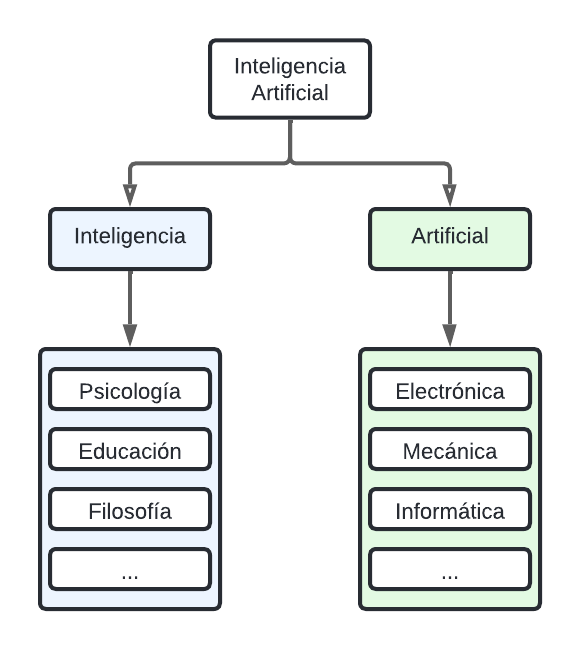
\includegraphics[scale=0.8, trim=0.5cm 0.5cm 0.5cm 0.5cm]{figs/artificial-vs-intelligence.png}
	\caption{\small"Inteligente" vs "Artificial". Elaboración Propia}
	\label{fig:etiqueta}
\end{figure}

Tras la Conferencia de Dartmouth organizada en 1956 por el matemático John McCarthy
junto con otro investigadores como Marvin Misnky, se definieron por primera vez las
bases de la inteligencia artificial:

\begin{quote}
	\textit{
		"El estudio procederá sobre la base de la conjetura de que cada aspecto
		del aprendizaje o cualquier otra característica de la inteligencia
		puede, en principio, ser descrito con tal precisión que se pueda crear
		una máquina capaz de simularlo." \citet{mccarthy2006proposal}
	}
\end{quote}

A lo largo de las decadas posteriores, el concepto de inteligencia artificial (IA) podrá
definirse entorno a 3 interpretaciónes de distintos sectores:

\begin{itemize}
	\item Desde la perspectiva de la IA clásica, desarrollada principalmente por
	      los campos de las matemáticas e informática, la inteligencia artificial se
	      concibe como un conjunto de algoritmos predefinidos, reglas de inferencia y
	      razonamientos lógicos que buscan tomar decisiones, realizar tareas complejas
	      o resolver problemas de manera autónoma. El objetivo de la IA clásica es
	      resolver tareas como encontrar el camino más corto entre dos puntos o
	      seleccionar el movimiento con mayor probabilidad de éxito en un juego como
	      el ajedrez.

	\item Desde la perspectiva del aprendizaje automático, la inteligencia
	      artificial se define como una propiedad emergente de modelos matemáticos
	      complejos, cuya interpretación no se basa en una secuencia de pasos
	      predeterminada sino en las interacciones del modelo como conjunto. En este
	      caso, de forma similar a como un cuadro artistico emerge como consecuencia
	      del agrupamiento de trazos y colores adecuadamente posicionados, la IA
	      emergera como resultado de las interacciones entre diferentes entidades
	      matemáticas.  \footnote{Cabe señalar que, bajo este enfoque, la IA no puede
		      ser controlada de forma determinista, ya que los modelos matemáticos no
		      definen en su totalidad el comportamiento resultante de su aplicación.}

	\item Desde la perspectiva del campo de la cognición (interpretación que
	      utilizará de aquí en adelante), la inteligencia artificial
	      es un sistema que replica habilidades como el razonamiento, la resolución de
	      problemas, la toma de decisiones, el aprendizaje y la percepción de manera
	      similar a las funciones realizadas por el cerebro humano. Dado este enfoque,
	      el funcionamiento interno de la inteligencia no está explícitamente
	      definido, pues se considera que la "inteligencia" reside en el proceso de
	      resolución de problemas y no en los datos que contiene. Es decir, la
	      inteligencia se manifiesta en la metodologia con la que dicho sistema
	      "piensa", y no únicamente en la información que posee.

	      \begin{figure}[!hbp]
		      \centering
		      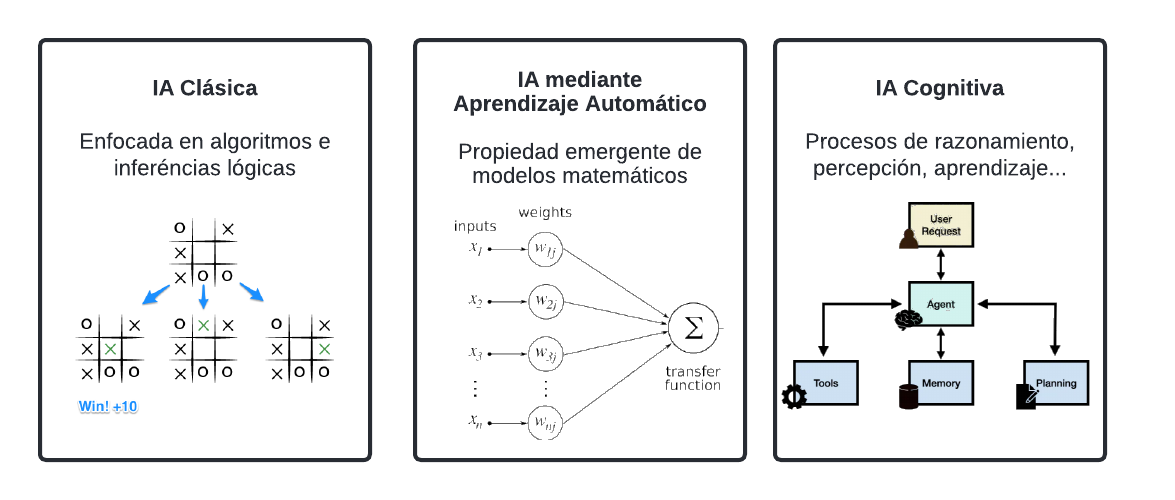
\includegraphics[scale=0.32, trim=0.9cm 0.9cm 0.9cm 0.9cm]{figs/AI-interpretations.png}
		      \caption{\small Interpretaciones de Inteligencia Artificial. Elaboración Propia}
		      \label{fig:etiqueta}
	      \end{figure}

\end{itemize}


El desarrollo de la inteligencia artificial ha dado paso a la investigación de
multiples areás sobre lo que se consideraba "inteligente" y como estos sectores
podian ser automatizados, esto es, convertirlos en elementos artificiales.
Entre las áreas de estudio destacadas encontramos investigaciones sobre la
representación del conocimiento, la inferencia, o la resolución de problemas.

De entre todas estas areas, la resolución de problemas destaca aun a día de hoy
como una de las propiedades mas dificiles de alcanzar. Esto se debe a que
resolver un problema, a diferencia de otras tareas, implica resolver multiples
subtareas que son faciles de para un humano pero a su vez dificilmente
automatizables. Como ejemplo, la tarea de distinguir los comentarios negativos
de los positivos en un foro de internet, resulta trivial de forma intuitiva, sin
embargo matices sutiles del lenguaje como la ironia, gracia, emoción o
exageración resultan imposibles de determinar en un conjunto de pasos que
ejecuta un algoritmo o maquina.

\begin{figure}[!hbp]
	\centering
	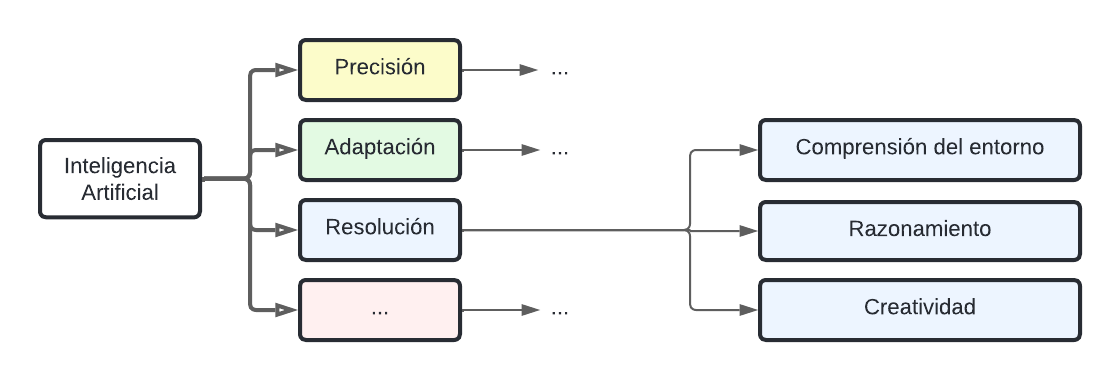
\includegraphics[scale=0.3, trim=0.5cm 0.5cm 0.5cm 0.5cm]{figs/AI-properties.png}
	\caption{\small Requisitos de la IA. Elaboración Propia}
	\label{fig:etiqueta}
\end{figure}

\section{Fundamentos de la IA Moderna}

Entre otras arquitecturas de inteligencia artificial, los Modelos Grandes de
Lenguaje (LLM por sus siglas en ingles), han destacado en los ultimos años por
su capacidad de adaptarse a multiples aplicaciones. Utilizando el enfoque de
inteligencia artificial basada en aprendizaje automático, estos modelos son
capaces de generar imagenes, entender matices del lenguaje como la ironia,
razonar matemáticamente o incluso generar modelos 3D a partir de descripciones
de un objeto.

Independientemente de su estructura interna, podemos razonar que estos sistemas
actuan de forma inteligente (acorde al razonamiento establecido en la sección
\ref{sec:artificial_intelligence}). Por esta razón, muchas empresas han adoptado
tecnologías de IA que les permiten ahorrar tiempo, esfuerzo y, en algunos casos,
mejorar la calidad de sus tareas. Entre estas tareas automatizadas se encuentra
la generación automática de texto, donde la IA recibe un \textit{prompt}, esto
es, una entrada en formato de texto que contiene las instrucciones que debe
seguir, y responde de forma automática. Esta respuesta puede utilizarse, por
ejemplo, para actualizar contenido en redes sociales o resumir textos largos.

\begin{figure}[!hbp]
	\centering
	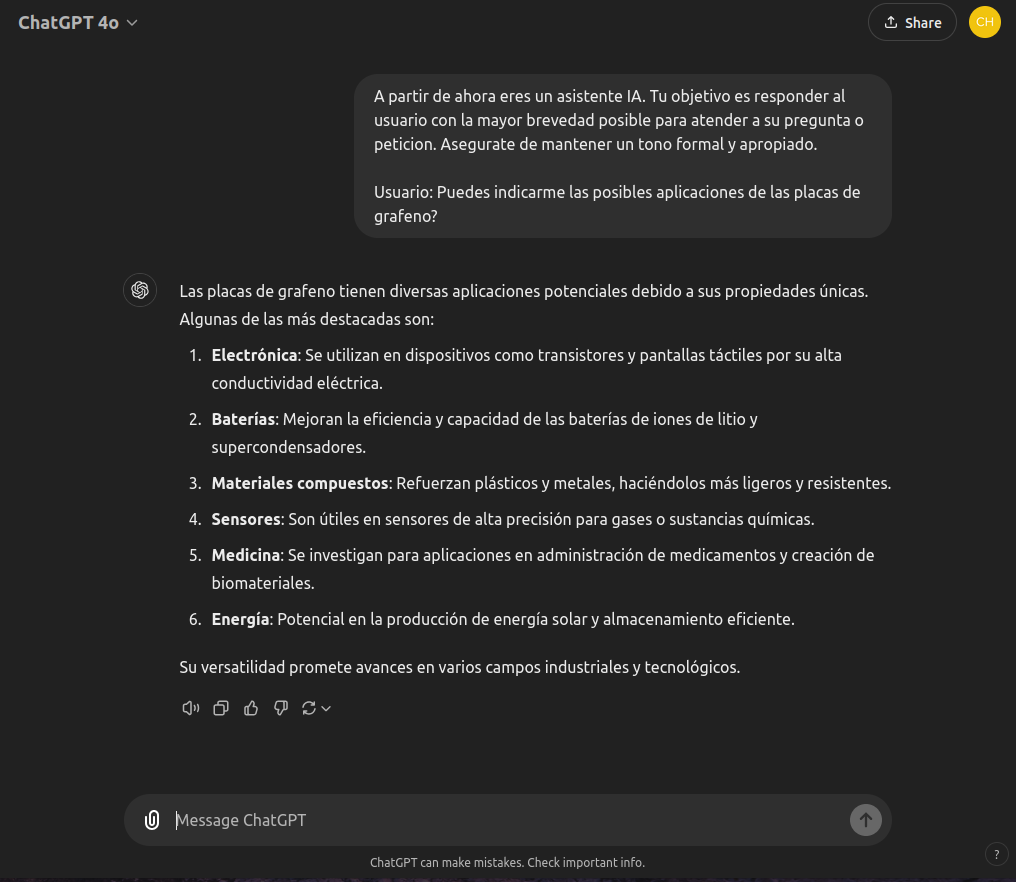
\includegraphics[scale=0.3]{figs/chatgpt.png}
	\caption{\small Interacción automatizada con usuario utilizando ChatGPT (modelo GPT-4o-mini). Elaboración Propia}
	\label{fig:etiqueta}
\end{figure}

Detrás de los modelos de lenguaje actuales subyacen arquitecturas avanzadas
basadas en redes neuronales profundas. A diferencia de otras tecnologías, estas
arquitecturas requieren un proceso intensivo de entrenamiento, optimización y
refinamiento a través de múltiples capas, con el fin de garantizar tanto su
robustez como su eficiencia. En este contexto, diferentes compañías proporcionan
servicios basados en cómo han refinado y optimizado dichas arquitecturas.

Un ejemplo es OpenAI, que ofrece acceso a sus modelos GPT a través de su
\href{https://openai.com/}{pagina web}. Los modelos más recientes de esta serie
destacan por su capacidad superior para la comprensión del lenguaje natural,
razonamiento y control en tareas complejas. En contraste, la empresa
\href{https://docs.anthropic.com/es/docs/about-claude/models}{Anthropic}, ofrece
proporciona acceso a sus modelos Claude Haiku, diseñados para ofrecer respuestas
rápidas y con un enfoque en la optimización de costos, según lo informado en su
plataforma en línea. Cada compañía, por tanto, implementa variaciones en el
diseño y entrenamiento de sus modelos, lo que conduce a distintas capacidades y
enfoques en el mercado de modelos de lenguaje.

Para aprovechar en su totalidad el potencial de los modelos de lenguaje (LLMs), surge
el concepto de Agente. Un agente es una tecnología diseñada para conectar a las
LLMs con diversos campos de aplicación. En esencia, un agente contiene una
inteligencia artificial capaz de razonar y tomar decisiones basadas en las
posibles acciones a implementar. Posteriormente, utiliza herramientas
preprogramadas en su arquitectura para traducir esos razonamientos en
aplicaciones concretas.

Estos agentes pasan por diversas fases de razonamiento, comúnmente denominadas
arquitecturas agénticas, que les permiten interactuar tanto con usuarios como
con otros objetos o incluso agentes. A lo largo de este proceso, el agente
evalúara la situación y ejecuta las acciones más adecuadas según las
herramientas disponibles en su estructura. Un ejemplo de esta tecnología se
encuentra en \textsc{Gemini Advanced}, un agente desarrollado por Google. Este
agente es capaz de procesar las solicitudes del usuario a través de comandos de
voz en un dispositivo móvil, y ejecuta las acciones pertinentes para cumplir con
la petición. La arquitectura de este agente le permite interpretar el lenguaje
natural del usuario y, utilizando las herramientas integradas en su sistema,
realizar las tareas necesarias de manera eficiente.

\begin{figure}[!hbp]
	\centering
	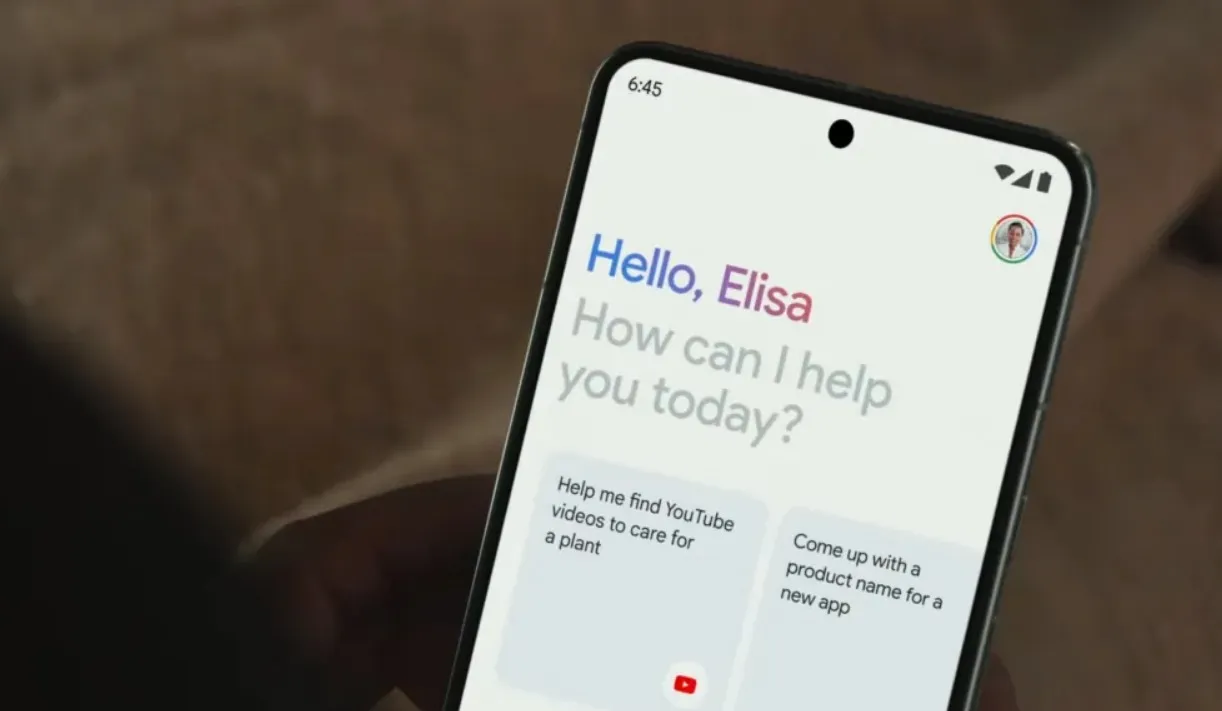
\includegraphics[scale=0.2]{figs/gemini-phone.png}
	\caption{\small Interacción movil con Gemini Advance. Fuente: \href{https://es.digitaltrends.com/computadoras/cosas-increibles-que-puedes-hacer-con-google-gemini-advanced/}{es.digitaltrends.com/}.}
	\label{fig:etiqueta}
\end{figure}

En la presente memoria se propone implementar una Máquina de Cognición y
Ejecución (MCE), esto es, una arquitectura agéntica que permita a una
inteligencia artificial interactuar con su entorno de manera generalista,
similar a \textsc{Gemini Advanced}.

En el siguiente capítulo, se abordarán los principales conceptos y tecnologias
relevantes para el diseño de arquitecturas agénticas. Se realizará una revisión
de las tecnologias actuales y sus capacidades cognitivas, analizando cómo se
diferencian los agentes de propósito general de la inteligencia general
artificial. Además, se explorarán las técnicas de comportamiento que permiten a
los AGI's tomar decisiones de forma autónoma y eficiente. Finalmente, se
examinará el estado actual de las arquitecturas cognitivas, enfocándose en sus
limitaciones y los avances que han permitido una mayor capacidad de razonamiento
y adaptabilidad en agentes de IA.
